\documentclass[a4paper,12pt]{article}
\usepackage{a4wide}
\usepackage{tikz}
\usetikzlibrary{calc}
\usepackage{hyperref}

\begin{document}
\pagestyle{empty}
\setlength{\parindent}{0em} 
\section*{FSM (Finite State Machine)}
Your task is to program the behavior of an entity called "fsm". This entity is declared in the attached file "fsm.vhdl" and has the following properties:

\begin{itemize}
\item Input: CLK with type std\_logic
\item Input: RST with type std\_logic
\item Input: INPUT with type std\_logic\_vector of length 2     
\item Output: OUTPUT with type std\_logic\_vector of length 2
\item Output: STATE with type fsm\_state
 
\end{itemize}

\begin{center}
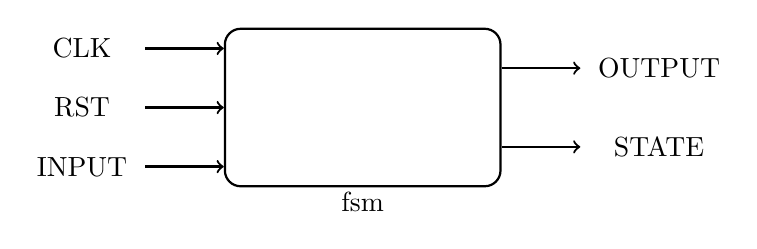
\begin{tikzpicture}
\draw node [draw,rectangle, minimum height=20mm, minimum width=35mm,rounded corners=2mm,thick](entity){};

\draw[->,thick] ($ (entity.west)+(-10mm,7.5mm) $) -- ($ (entity.west) +(0mm,7.5mm)$);
\draw node at ($ (entity.west)+(-18mm,7.5mm) $){CLK};

\draw[->,thick] ($ (entity.west)+(-10mm,0mm) $) -- ($ (entity.west) +(0mm,0mm)$);
\draw node at ($ (entity.west)+(-18mm,0mm) $){RST};

\draw[->,thick] ($ (entity.west)+(-10mm,-7.5mm) $) -- ($ (entity.west) + (0mm,-7.5mm)$);
\draw node at ($ (entity.west)+(-18mm,-7.5mm) $){INPUT};

\draw[->,thick] ($(entity.east)+(0mm,+5mm) $) -- ($(entity.east)+(+10mm,+5mm)$);
\draw node at ($ (entity.east) + (20mm,+5mm) $){OUTPUT};

\draw[->,thick] ($(entity.east)+(0mm,-5mm) $) -- ($(entity.east)+(+10mm,-5mm)$);
\draw node at ($ (entity.east) + (20mm,-5mm)$){STATE};

\draw node at ($ (entity) - (0,12mm)$){fsm};

\end{tikzpicture}
\end{center}

Do not change the file "fsm.vhdl".
\\

The "fsm" entity shall have the behavior of a deterministic finite state machine with the following constraints:
\begin{itemize}
\item Behavior according to state diagram as seen in Figure \ref{state_image}. The input to transit to the next state and the output in the next state is labelled on the edges.
\item Transitions with rising edge of the clock (port CLK, this is a square-wave clock signal).
\item Synchronous design: all new outputs (port STATE and port OUTPUT) have to be set with rising edges of the clock.
\item The current state has to be output at the output port STATE.
\item At synchronous reset (port RST=1, rising edge of clock port CLK) the state machine is set to an initial state: STATE= START, OUTPUT= 00
\end{itemize}
\vspace{0.2cm}

This behavior has to be programmed in the attached file "fsm\_beh.vhdl".
\\

The type fsm\_state is declared in the attached "fsm\_package.vhdl" file. The needed package to use this type is already imported in the attached "fsm\_beh.vhdl" and "fsm.vhdl". 
\\


To turn in your solution write an email to %%SUBMISSIONEMAIL with Subject "Result Task %%TASKNR" and attach your file "fsm\_beh.vhdl".

\vspace{0.7cm}

Good Luck and May the Force be with you.

\newpage

\begin{figure}[ht]
	\centering
        \includegraphics[width=\textwidth,height=\textheight,keepaspectratio]{%%STATECHART}
	\caption{State diagram, the edges are labelled Input / Next Output}
	\label{state_image}
\end{figure}

\end{document}
